\chapter{Desarrollo del trabajo}

En este capítulo se realizará un estudio detallado del estado del arte para posteriormente detallar las distintas fases de desarrollo y los problemas que han surgido con sus respectivas soluciones.

\section{Desarrollo profundo del estado del arte}

Este trabajo es la continuación de mi anteior TFG donde traté el tema de la renderización de conjuntos de datos volumétricos, este trabajo está dirigido al tratamiento de este conjunto de datos.

Un conjunto de datos volumétrico o campo escalar 3D está representado por una función $R^{3} \rightarrow R$. En otras palabras, se trata de un conjunto de datos representado por una matriz tridimensional, donde cada elemento de esta matriz se puede denominar vóxel y es importante tener claro que el valor de este no es un color sino un valor como tal que posteriormente se renderizará con un color y una transparencia según una función de transferencia. Es ahí donde erradica la separación conceptual entre modelado y visualización de un conjunto de datos volumétrico.

El flujo a la hora de representar un conjunto de datos volumétricos sería el siguiente:

\begin{itemize}
	\item Obtención de imágenes
	\item Filtrado
	\item Segmentación
	\item Visualización
\end{itemize}

Durante el TFG traté el último de los pasos y en este TFM comentaré las distintas opciones del primero y trabajaré en técnicas del segundo y el tercero aplicadas a esculturas de madera policromadas.

\subsection{Obtención de imágenes}

Existen diversas técnicas de obtención de imágenes volumétricas. En esta sección se describirán las dos técnicas más usadas actualmente y se realizará una comparación entre ellas. No se han incluido técnicas como el PET, SPECT o ecografía pues necesitan de contrastes que no se podrían aplicar en una escultura si se quiere preservar su estado.

\subsubsection{Tomografía Computarizada}

La Tomografía Computarizada (TC o CT en inglés) fue la primera de las técnicas que surgió para la obtención de datos volumétricos pero ha ido evolucionando hasta el día de hoy como se detalló en la introducción.

\begin{figure}[H]
	\centering
	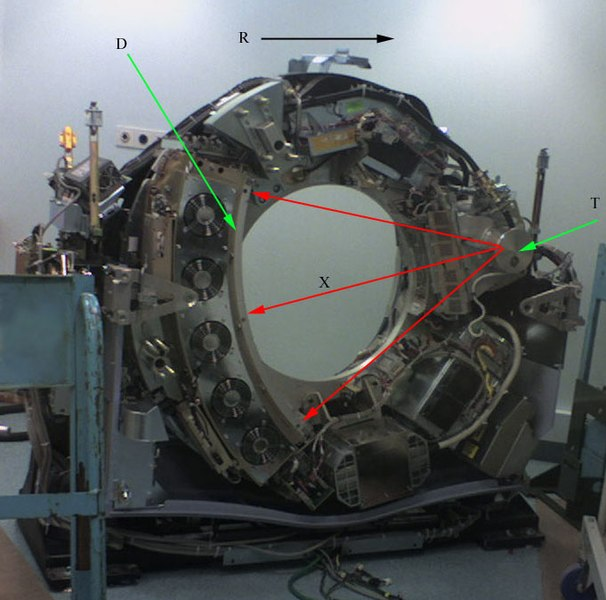
\includegraphics[width=9cm]{imagenes/desarrollo/tc}
	\caption{Escáner TC sin la carcasa, por lo que se puede ver sus componentes internos. T: Tubo rayos X, D: Detectores rayos X, X: Haces de rayos X y R: \textit{Gantry}. Imagen extraída de: \url{https://en.wikipedia.org/wiki/File:Ct-internals.jpg}}
	\label{fig:desarrollo/tc}
\end{figure}

Los parámetros utilizados en una TC son los siguientes:

\begin{itemize}
	\item \textbf{Resolución espacial} (número de cortes, píxeles por corte y distancia entre vóxeles): Si la resolución es más alta los datos serán más ruidosos si la dosis de radiación se mantiene.
	\item \textbf{Dosis de radiación}: Si la dosis de radiación es mayor se conseguirá mejor ratio señal-ruido y las imágenes podrán ser de mayor resolución sin que el ruido sea un problema.
	\item \textbf{\textit{Gantry tilt}} (sistema de rotación emisor/receptor): Se puede adaptar el \textit{gantry tilt} para una parte específica a examinar.
\end{itemize}

Los valores de intensidad de las imágenes extraídas se encuentran en unidades Hounsfield (HU). Que es una unidad de medida normalizada que hace que un tejido tenga ese valor sean cuales sean los parámetros del escáner.

\subsubsection{Imagen por Resonancia Magnética}

La Imagen por Resonancia Magnética (IRM o MRI en inglés) es una técnica en la que, a diferencia de la TC donde se usa radiación ionizante, se usan campos mágnéticos para diferenciar los distintos materiales del objeto escaneado, específicamente la ocurrencia del núcleo de hidrógeno que son capaces de absorber y emitir radio frecuencia cuando se colocan en un campo magnético externo \cite{mcrobbie10}.

\begin{figure}[H]
	\centering
	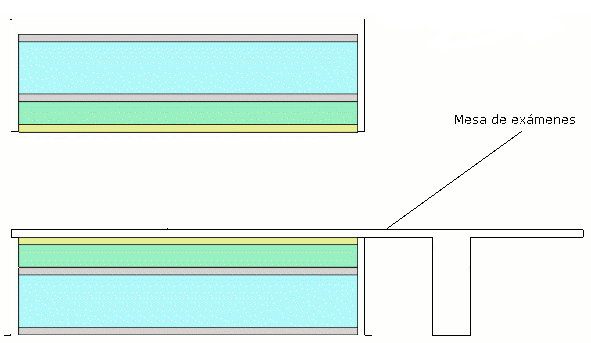
\includegraphics[width=12cm]{imagenes/desarrollo/irm-longitudinal}
	\caption{Esquema de un escáner IRM (Sección Longitudinal). Imagen extraída de: \url{https://en.wikipedia.org/wiki/File:Mri_scanner_schematic_labelled.svg}}
	\label{fig:desarrollo/irm-longitudinal}
\end{figure}

\begin{figure}[H]
	\centering
	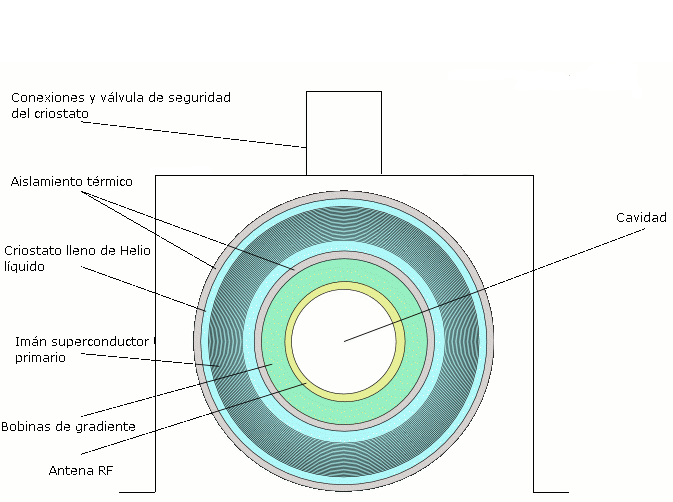
\includegraphics[width=12cm]{imagenes/desarrollo/irm-axial}
	\caption{Esquema de un escáner IRM (Sección Axial). Imagen extraída de: \url{https://en.wikipedia.org/wiki/File:Mri_scanner_schematic_labelled.svg}}
	\label{fig:desarrollo/irm-axial}
\end{figure}

El campo magnético alinea los momentos magnéticos de los núcleos atómicos de hidrógeno en dirección paralela y anti-paralela. 

A continuación se emite radiación electromagnética a un pulso de radiofrecuencia determinado. Algunos núcleos que se encuentran en dirección paralela pasarán a anti-paralela y al volver a su dirección original perderán energía en forma de fotones que podrán ser detectados. 

Estos dos tiempos, T1 (\textit{phase}) y T2 (\textit{dephase}) son medidos. Para obtener T1 hay que ver el valor en la gráfica de relajación longitudinal al 63\% y para obtener T2 hay que hacer lo mismo en la gráfica de relajación transversal al 37\% \cite{relaxation}.

\begin{figure}[H]
	\centering
	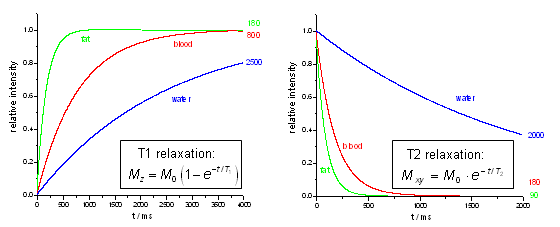
\includegraphics[width=12cm]{imagenes/desarrollo/relajacion-longitudinal-transversal}
	\caption{A la izquierda gráfica de la relajación longitudinal (crecimiento logarítmico) y a la derecha gráfica de la relajación transversal (crecimiento exponencial). Imagen extraída de: \url{http://www.nmr.uni-duesseldorf.de/main/mtheorie_3_e.html}}
	\label{fig:desarrollo/relajacion-longitudinal-transversal}
\end{figure}

\subsubsection{Comparación entre TC e IRM}

Las principales diferencias entre ambas técnicas son las siguientes:

\begin{itemize}
	\item La IRM obtiene imágenes de menor resolución que la TC.
	\item La IRM proporciona un mayor contraste entre tejidos poco densos.
	\item Los datos obtenidos con una TC son más entendibles por médicos mientras que los obtenidos con una IRM por radiólogos.
	\item El tiempo y coste de escaneo de una IRM es mayor que el de una TC.
	\item Los datos obtenidos con una TC se encuentran en unidades normalizadas mientras que los obtenidos con una IRM variarán dependiendo de los parámetros del escáner.
\end{itemize}

Al necesitar unos \textit{presets} con los que se pueda visualizar la escultura sin necesidad de que el usuario edite la función de transferencia, el último punto nos haría decantar por la TC. Además gracias a esta podremos obtener imágenes de mayor resolución. El único punto en contra en esta elección es que el contraste entre materiales de baja densidad (como la madera) no será tan distinguible como con la IRM.

\subsection{Filtrado}

Lala

\subsection{Segmentación}

Lala

\section{Fases de desarrollo}

Lala

\section{Problemas y soluciones}

Lala